%% 美赛模板:正文部分

\documentclass[12pt]{article}  % 官方要求字号不小于 12 号,此处选择 12 号字体

% 本模板不需要填写年份,以当前电脑时间自动生成
% 请在以下的方括号中填写队伍控制号
\usepackage[2124173]{easymcm}  % 载入 EasyMCM 模板文件
\problem{F}  % 请在此处填写题号
\usepackage{mathptmx}  % 这是 Times 字体,中规中矩 
\usepackage{cite}
\title{An ICM Paper Made by Team 2124173}  % 标题

% 如需要修改题头(默认为 MCM/ICM),请使用以下命令(此处修改为 MCM)
%\renewcommand{\contest}{MCM}

% 文档开始
\begin{document}
	
% 此处填写摘要内容
\begin{abstract}
In today's era of rapid development, a healthy and sustainable higher education system 
is a must for a country to stay ahead of the curve. It can produce top talents, develop 
cutting-edge technologies and improve social productivity. In this paper, we assess the
 health of a country's higher education system by using \textbf{Analytic Hierarchy Process}
  and \textbf{Fuzzy Synthetic Evaluation} and analyze the specific situation in Brazil.

We divided seven factors affecting the degree of health by stratification and applied Analytic Hierarchy Process 
to calculate the initial weights of each factor. Using the Fuzzy Synthetic Evaluation, the health status was first 
divided into five degrees, and then the data of each influencing factor was divided into five classes. Each grade 
corresponds to a determined \textbf{single-factor evaluation vector}, from which an evaluation matrix is derived. 
The comprehensive evaluation weight matrix was calculated by combining the preliminary weights, and the final score 
was obtained by weighting it, and finally the results were obtained according to the health degree according to the 
final score.

The health level in the third or fourth class is considered to be improved. Applying the model to the United States, 
Germany, Korea and Brazil, it was found that Brazil was in the third class. We analyzed the reasons for Brazil's poor 
health status, identified the weaker parts of the data on the influencing factors, and proposed a reasonable vision. 
After combing with health level assessment model, we found that its health level became the second class. The phenomenon 
indicated the validity of the vision. At the same time, we proposed a series of policies (such as reducing the number of 
places reserved in the \textbf{Brazilian higher education enrollment mandatory bias decree policy}) (a series of practical 
and feasible) and a specific implementation schedule.

In the process of implementing multiple policies, the relative strengths of the policies were set, and the correlations 
between the policies and the seven factors were determined, and the \textbf{growth coefficients} for each factor were 
obtained for all policies. The factors with higher growth coefficients were found to be the weaker parts of Brazil, 
indicating that the policy implementation was reasonable and effective. 

Finally, our analysis shows that the implementation of the policy will have a significant impact on students from 
low-income families, public and private universities, and the distribution of social resources. Worse still, it is 
very difficult to change due to the economic and wealth divide.



    % 美赛论文中无需注明关键字。若您一定要使用,
    % 请将以下两行的注释号 '%' 去除,以使其生效
\vspace{5pt}
\textbf{Keywords}: AHP,  Fuzzy Synthetic Evaluation, Higher Education Health Condition.

\end{abstract}

\maketitle  % 生成 Summary Sheet

\tableofcontents  % 生成目录


% 正文开始
\section{Introduction}
\subsection{Problem Background}
Education is a national issue, and the degree of health and sustainability of the higher education system is also a good indicator of the health of the nation. The health of the higher education system is linked to cost, access, equity, funding, the value of degrees, and the quality of education. 

The health of the higher education system can greatly affect subsequent national learning when the overall level of national education is higher than that of primary and secondary education. People who have experienced healthy higher education will also repay the country's investment in education in all aspects of society. 

However, each country's higher education system has its weaknesses, and it is essential to be able to propose timely adjustments. An attempt has been made to develop a model that can always assess the degree of health and sustainability of the education system. With this understanding, our group proposes a model for assessing the health of national higher education systems that provides a good assessment score for any country, while also reflecting current deficiencies for policy development.
\subsection{Our work}

\begin{enumerate}[\bfseries 1.]
    \item Develop and validate a model or suite of models to assess the health of any nation’s system of higher education. 
    \item Apply our models to several countries, and then select a nation whose system of higher education has room for improvement.
    \item Propose an attainable and reasonable vision for our selected nation’s system.
    \item Use our models to measure the health of both the current system and proposed, healthy, sustainable system for selected nation.
    \item Propose targeted policies and an implementation timeline.
    \item Use our models to assess the effectiveness of policies.
    \item Discuss the real-world impacts.
\end{enumerate}

\section{Preparation of the Models}
\subsection{Data Bank}
\newpage
\begin{table}[htp]
		\begin{center}
	\begin{tabular}{|c|c|c|c|}
		\hline
		Country       & Education index & Research index & Times Number of Top 500 colleges \\ \hline
		United States & 48.5808         & 45.6136        & 118                        \\ \hline
		Germany       & 43.1512         & 45.5902        & 43                         \\ \hline
		South Korea   & 48.6000         & 50.5700        & 10                         \\ \hline
		Brazil        & 50.9500         & 51.4000        & 2                          \\ \hline
	\end{tabular}
		\end{center}
\end{table}

\begin{table}[htp]
	\begin{center}
	\begin{tabular}{|c|c|c|}
		\hline
		Country        & College Enrollment Rate & \begin{tabular}[c]{@{}c@{}}2014 Expenditure on higher education as a percentage\\  of government expenditure on education\end{tabular} \\ \hline
		United  States & 88.2                    & 27.50                                                                                                                                  \\ \hline
		Germany        & 70.2                    & 26.59                                                                                                                                  \\ \hline
		South Korea    & 94.3                    & 20.76                                                                                                                                  \\ \hline
		Brazil         & 51.3                    & 19.27                                                                                                                                  \\ \hline
	\end{tabular}
	\end{center}
\end{table}

\begin{table}[htp]
	\begin{center}
	\begin{tabular}{|c|c|c|}
		\hline
		Country       & \begin{tabular}[c]{@{}c@{}}2017 Proportion of all international students\\  to the number of students in higher education\end{tabular} & \begin{tabular}[c]{@{}c@{}}2017 Expected years of schooling \\ for all students in higher education\end{tabular} \\ \hline
		United States & 5.18                                                                                                                                   & 4.00                                                                                                             \\ \hline
		Germany       & 8.37                                                                                                                                   & 3.26                                                                                                             \\ \hline
		South Korea   & 2.26                                                                                                                                   & 4.61                                                                                                             \\ \hline
		Brazil        & 0.24                                                                                                                                   & 2.40                                                                                                             \\ \hline
	\end{tabular}
	\end{center}
\end{table}
\subsection{Notations}
The primary notations used in this paper are listed in Table \ref{tb:nnn} and Table \ref{tb:ooo}.

\begin{table}[htbp]
\begin{center}
	\caption{New Notations1}
	\begin{tabular}{cl} % 控制表格的格式
		\toprule
	\multicolumn{1}{m{3cm}}{\centering Symbol}
	&\multicolumn{1}{m{12cm}}{\centering Definition}\\
		\midrule
		$I_1$&Higher education enrollment rate\\
		$I_2$&   Higher education as a percentage of government spending on education\\
		$I_3$&   Number of Top 500 Colleges\\
		$I_4$&   Teaching index\\
		$I_5$&   Research index\\
		$I_6$&   Proportion of international students\\
		$I_7$&   Expected length of education\\
		$N$&   Correlation Matrix\\
		$B$&   Fuzzy Synthetic Evaluation Weight Matrix\\
		$W$&   Relative implementation strength\\
		$\omega$&   Weight Vector of Evaluation\\
		\bottomrule
	\end{tabular}\label{tb:nnn}
\end{center}
\end{table}
\newpage
\begin{table}[htp]
	\begin{center}
		\caption{New Notations2}
		\begin{tabular}{cc} % 控制表格的格式
			\toprule
			\multicolumn{1}{m{3cm}}{\centering Symbol}
			&\multicolumn{1}{m{6cm}}{\centering Definition}\\
			\midrule
		$V_1$&   Very healthy\\
		$V_2$&   Healthy\\
		$V_3$&   Normal\\
		$V_4$&   Less healthy\\
		$V_5$&   Unhealthy\\
			\bottomrule
		\end{tabular}\label{tb:ooo}
	\end{center}
\end{table}

\section{The Models}
\subsection{Model 1}
\subsubsection{Establish by using Analytic Hierarchy Process\cite{8}}
The health of a country's higher education system is influenced by the above seven main factors. We choose the hierarchical analysis method to find the weight of each factor.

1. Establish a hierarchical model
Goal level G, health status of higher education system; Criteria level C, popularity rate, government economic input, quality university resources, degree of education; Alternative level A, enrollemtn rate, Higher education as a percentage of government spending on education, Number of top 500 colleges, Teaching Index, Research index, Proportion of international students, expected length of education.

The detail can be shown in Figure \ref{fig:overall}: %\eqref为交叉引用
\begin{figure}[htbp]
	\centering
	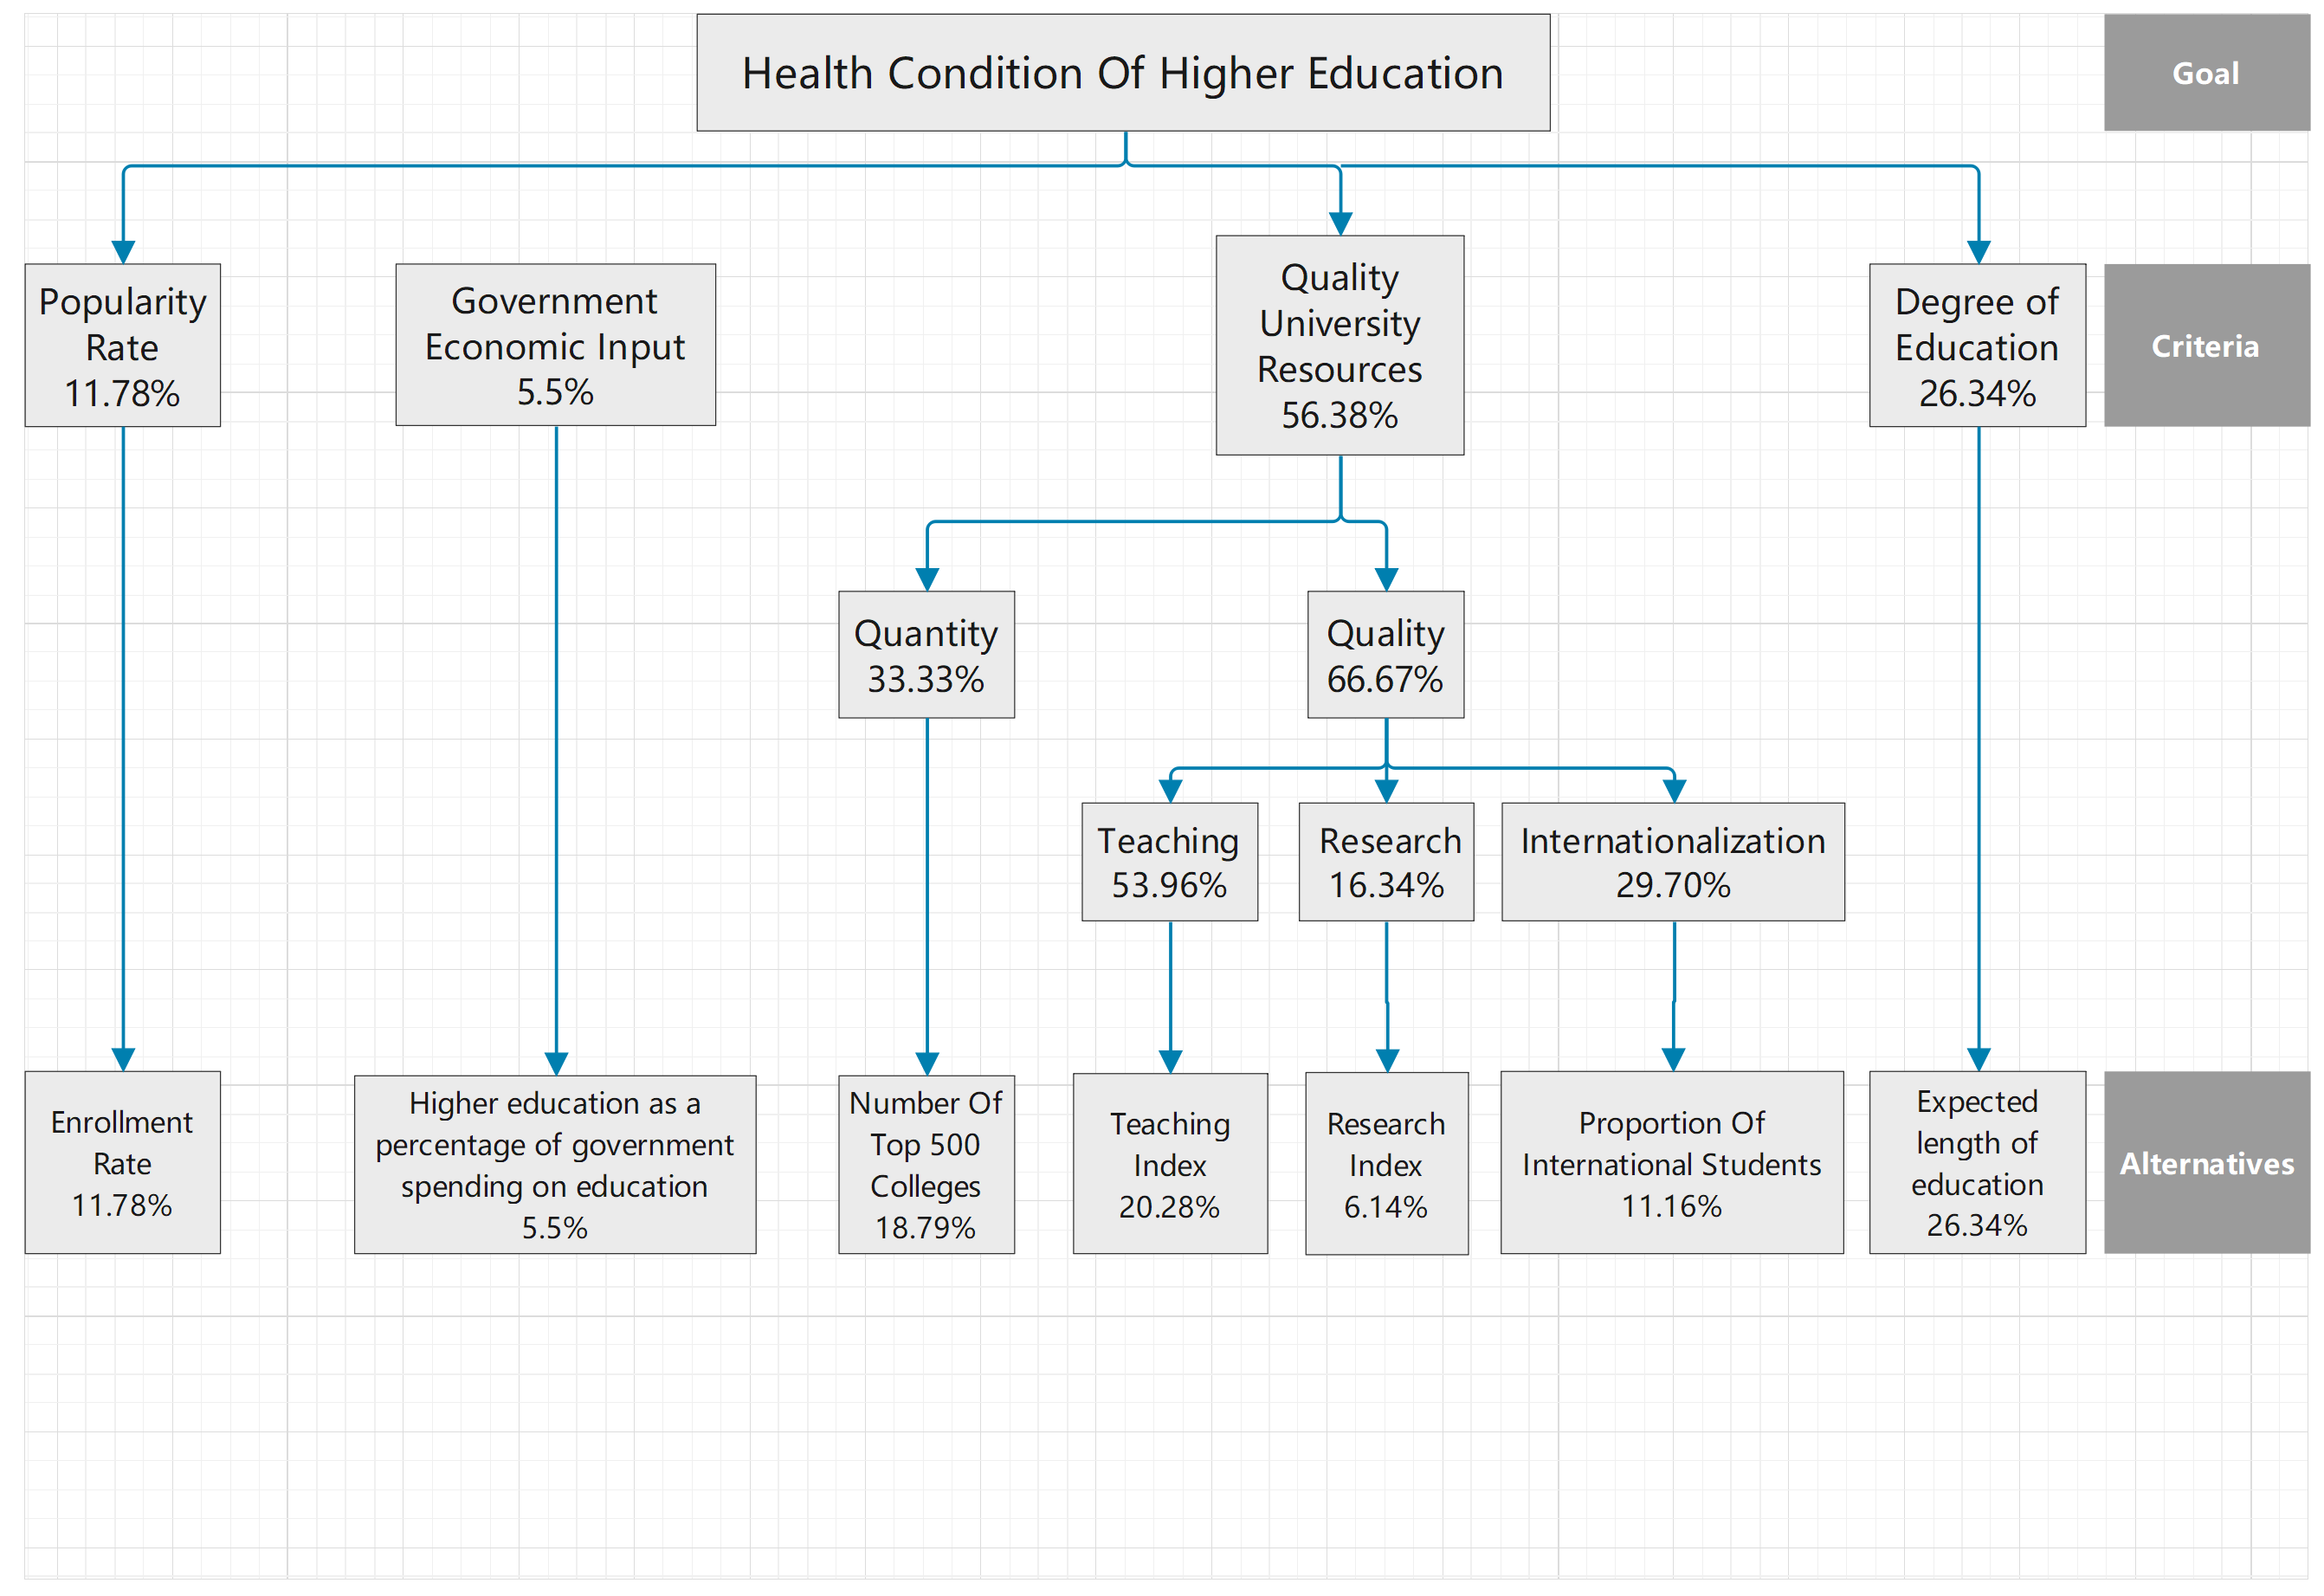
\includegraphics[width=.9\textwidth]{model relative.PNG}
	\caption{data relationship}\label{fig:overall}
\end{figure}

2. Construct the comparison matrix between the factors.

The first level of comparison matrix is  \eqref{eq:aaa}:
\begin{equation}\label{eq:aaa}%label为交叉引用供号准备
M_1=\begin{pmatrix}
1&3&\frac{1}{5}&\frac{1}{3}\\
\frac{1}{3}&1&\frac{1}{7}&\frac{1}{5}\\
5&7&1&3\\
3&5&\frac{1}{3}&1
\end{pmatrix}
\end{equation}

The first layer weight vector is \eqref{eq:bbb}:
\begin{equation}\label{eq:bbb}%label为交叉引用供号准备
\omega_1=(0.1178,0.055,0.5638,0.2634)
\end{equation}

The second level of comparison matrix is Matrix \eqref{eq:ccc}:
\begin{equation}\label{eq:ccc}%label为交叉引用供号准备
M_2=\begin{pmatrix}
1&\frac{1}{2}\\
2&1\\
\end{pmatrix}
\end{equation}

The second layer weight vector is \eqref{eq:ddd}:
\begin{equation}\label{eq:ddd}%label为交叉引用供号准备
\omega_2=(0.3333,0.6667)
\end{equation}

The third level of comparison matrix is Matrix \eqref{eq:eee}:
\begin{equation}\label{eq:eee}%label为交叉引用供号准备
M_3=\begin{pmatrix}
1&3&2\\
\frac{1}{3}&1&\frac{1}{2}\\
\frac{1}{2}&2&1\\
\end{pmatrix}
\end{equation}

The third layer weight vector is \eqref{eq:fff}:
\begin{equation}\label{eq:fff}%label为交叉引用供号准备
\omega_3=(0.5396,0.1634,0.2970)
\end{equation}

3. Consistency Test

Through solving the $M_1$ and $M_3$ eigenvalues, we get:

$$
\lambda_{1max}=4.1170,
\quad\lambda_{3max}=3.0092
$$

Through consistency indicators $CI$\eqref{eq:ggg}:
\begin{equation}\label{eq:ggg}%label为交叉引用供号准备
CI=\frac{\lambda_{max}-m}{m-1}
\end{equation}

We get:
$$
CI_1=0.0390,\quad CI_3=0.0046
$$

Through consistency rate $CR$\eqref{eq:hhh} 
\begin{equation}\label{eq:hhh}%label为交叉引用供号准备
CR=\frac{CI}{RI}
\end{equation}

and Table \ref{tb:mmm} 
\begin{table}[htbp]
	\centering
	\caption{Random consistency index}
	\begin{tabular}{l|lllllllllll} % 控制表格的格式
		\toprule
		$n$\cite{7} &1&2&      3&   4&   5&   6&   7&   8&   9&  10\\
		\midrule
        $RI$&  0&  0&  0.58&  0.90&  1.12&  1.24&  1.32&  1.41&  1.45&  1.49\\
		\bottomrule
	\end{tabular}\label{tb:mmm}
\end{table}
\newpage
We get:

$$
CR_{1}=0.043,
\quad CR_3=0.0079
$$

All three matrices pass the consistency test.

Through Equation \eqref{eq:iii}:
\begin{equation}\label{eq:iii}%label为交叉引用供号准备
\omega=\omega_1\omega_2\omega_3
\end{equation}

$\omega$ is the final weight vector derived using hierarchical analysis.
$$
\omega=(0.1178,0.055,0.1879,0.2028,0.0614,0.1116,0.2634)
$$
\subsection{Model 2}
\subsubsection{Establish by using Fuzzy Synthetic Evaluation}
To establish a system of evaluating indicators of the health of a country's higher education system based on the factors that affect its health status.

1.Defining the set of indicators
$$I=(I_1,I_2,I_3,I_4,I_5,I_6,I_7)$$

*The Definitions are shown in Table \ref{tb:nnn}.

2.Establishing evaluation levels:

$$V=(V_1,V_2,V_3,V_4,V_5)$$

*The Definitions are shown in Table \ref{tb:ooo}.

According to the given data, they were evaluated according to the following classification criteria Table \ref{tb:sss} and scoring criteria Table \ref{tb:vvv}.
\begin{table}[htp]
	\caption{Classification Criteria}
	\begin{tabular}{|c|c|c|c|c|c|c|}
		\hline
		& Factors                      & Level 1          & Level 2 & Level 3 & Level 4 & Level 5          \\ \hline
		Num      & Employment rate              & \textgreater{}80 & 80-60   & 60-40   & 40-20   & 20-0             \\ \hline
		|Num-25| & Expenditure/GDP              & 0-3              & 3-6     & 6-9     & 9-12    & \textgreater{}12 \\ \hline
		Num      & Number of Top 500 colleges   & \textgreater{}45 & 45-30   & 30-15   & 15-5    & 5-0              \\ \hline
		Num      & Teaching index               & \textgreater{}50 & 50-40   & 40-30   & 30-20   & 20-0             \\ \hline
		Num      & Research index               & \textgreater{}50 & 50-40   & 40-30   & 30-20   & 20-0             \\ \hline
		|Num-25| & International students \%    & 0-2              & 2-4     & 4-6     & 6-8     & \textgreater{}8  \\ \hline
		Num      & Expected length of education & \textgreater{}5  & 5-4     & 4-3     & 3-2     & 2-0              \\ \hline
	\end{tabular}\label{tb:sss}
\end{table}

*Note: If the value is the value at the demarcation, it is classified as one step to the right of the demarcation.
\begin{table}[htbp]
	\caption{Scoring criteria}
	\begin{center}
	\begin{tabular}{|c|c|c|c|c|c|}
		\hline
		& Very healthy & Healthy & Normal & Less healthy & Unhealthy \\ \hline
		Level 1 & 0.5          & 0.3     & 0.2    & 0            & 0         \\ \hline
		Level 2 & 0.2          & 0.5     & 0.2    & 0.1          & 0         \\ \hline
		Level 3 & 0.1          & 0.2     & 0.4    & 0.2          & 0.1       \\ \hline
		Level 4 & 0            & 0.1     & 0.2    & 0.5          & 0.2       \\ \hline
		Level 5 & 0            & 0       & 0.2    & 0.3          & 0.5       \\ \hline
	\end{tabular}\label{tb:vvv}
	\end{center}
\end{table}

And the evaluation matrix $R$=$(r_{ij})_{7\times5}$ is obtained: Table \ref{tb:ppp}
 \begin{table}[htp]
	\begin{center}
		\caption{Evaluation matrix}		
	\begin{tabular}{l|lllll}
		\hline
		\multicolumn{1}{c|}{} & $V_1$ & $V_2$ & $V_3$ & $V_4$ & $V_5$ \\ \hline
		$I_1$                 & $r_{11}$ & $r_{12}$ & $r_{13}$ & $r_{14}$ & $r_{15}$ \\
		$I_2$                  & $r_{21}$ & $r_{22}$ & $r_{23}$ & $r_{24}$ & $r_{25}$ \\
		$I_3$                  & $r_{31}$ & $r_{32}$ & $r_{33}$ & $r_{34}$ & $r_{35}$ \\
		$I_4$                  & $r_{41}$ & $r_{42}$ & $r_{43}$ & $r_{44}$ & $r_{45}$ \\
		$I_5$                  & $r_{51}$ & $r_{52}$ & $r_{53}$ & $r_{54}$ & $r_{55}$ \\
		$I_6$                  & $r_{61}$ & $r_{62}$ & $r_{63}$ & $r_{64}$ & $r_{65}$ \\
		$I_7$                  & $r_{71}$ & $r_{72}$ & $r_{73}$ & $r_{74}$ & $r_{75}$ \\ \hline
	\end{tabular}\label{tb:ppp}
		\end{center}
\end{table}

3.The weight vector of evaluation factors is Equation \eqref{eq:qqq}:
\begin{equation}\label{eq:qqq}
\omega=(0.1178,0.055,0.1879,0.2028,0.0614,0.1116,0.2634)
\end{equation}

The synthetic fuzzy integrated evaluation result vector is
$B=b_i(i=1,2,...,5)$
$$B=\omega R=(b_1,b_2,b_3,b_4,b_5)$$

4.Weighted processing fuzzy evaluation model to get the final score$F$:\ref{eq:rrr}
\begin{equation}\label{eq:rrr}
F=5\times b_1+4\times b_2+3\times b_3+2\times b_4+1\times b_5
\end{equation}

The table corresponding to the score and health condition is as follows:
Table \ref{tb:ttt}
\begin{table}[htp]
	\begin{center}
	\caption{Scores and Health Condition}
	\begin{tabular}{|l|l|}
		\hline
		Health condition & Score   \\ \hline
		Very healthy     & (4,5{]} \\ \hline
		Healthy          & (3,4{]} \\ \hline
		Normal           & (2,3{]} \\ \hline
		Less healthy     & (1,2{]} \\ \hline
		Unhealthy        & (0,1{]} \\ \hline
	\end{tabular}\label{tb:ttt}
		\end{center}
\end{table}

\section {Model Applications}

The statistics of the seven influencing factors from the United States, Germany, Korea, and Brazil were brought into the above model, and the final scores and health grades are shown in Table \ref{tb:uuu} and Figure \ref{fig:bbb}.

\begin{figure}[htp]
	\centering
	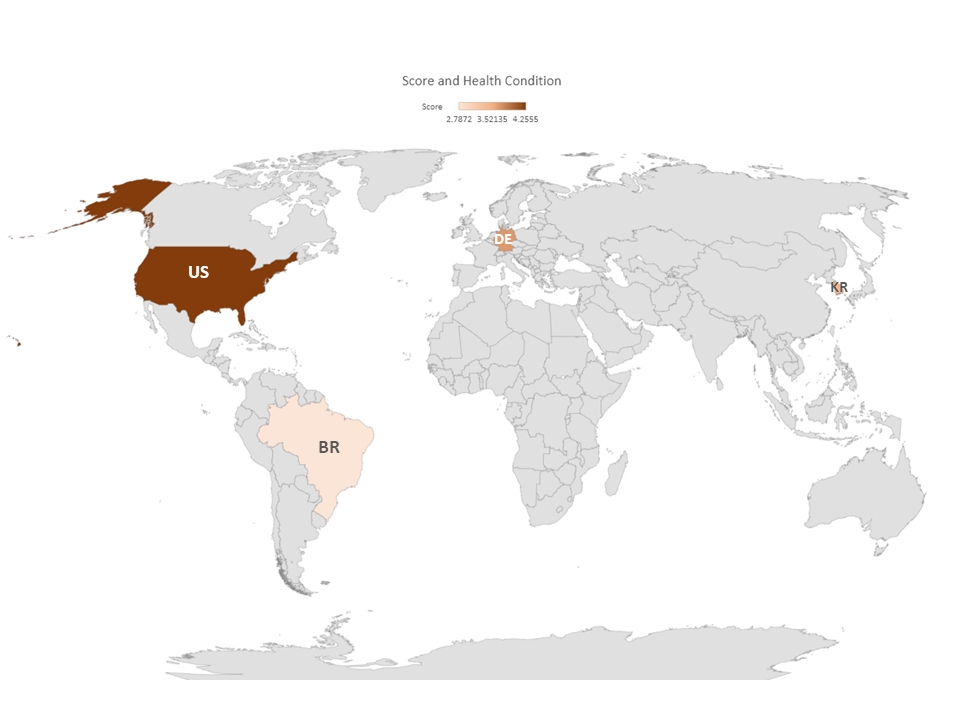
\includegraphics[width=.8\textwidth]{Score and Health Condition.PNG}
	\caption{Score and Health Condition}\label{fig:bbb}
\end{figure}

\begin{table}[htp]
	\caption{Score and Health Condition}
	\begin{center}
	\begin{tabular}{|l|l|l|}
		\hline
		Country       & Score  & Health Condition \\ \hline
		United States & 4.2555 & Very healthy     \\ \hline
		Germany       & 3.6722 & Healthy          \\ \hline
		South Korea   & 3.4099 & Normal           \\ \hline
		Brazil        & 2.7872 & Less healthy     \\ \hline
	\end{tabular}\label{tb:uuu}
	\end{center}
\end{table}
We generally consider that the higher education system in countries with average and below average health needs to be improved, and as seen in Table \ref{tb:uuu}, the higher education system in Brazil needs to be improved.

\section {Presenting the vision}

The proportion of existing influencing factors in Brazil and Eight years after presenting the vision, we expect the ratios to be as shown in Figure \ref{fig:ccc}.
\newpage
\begin{figure}[htp]
	\centering
	\begin{subfigure}[b]{.4\textwidth}
		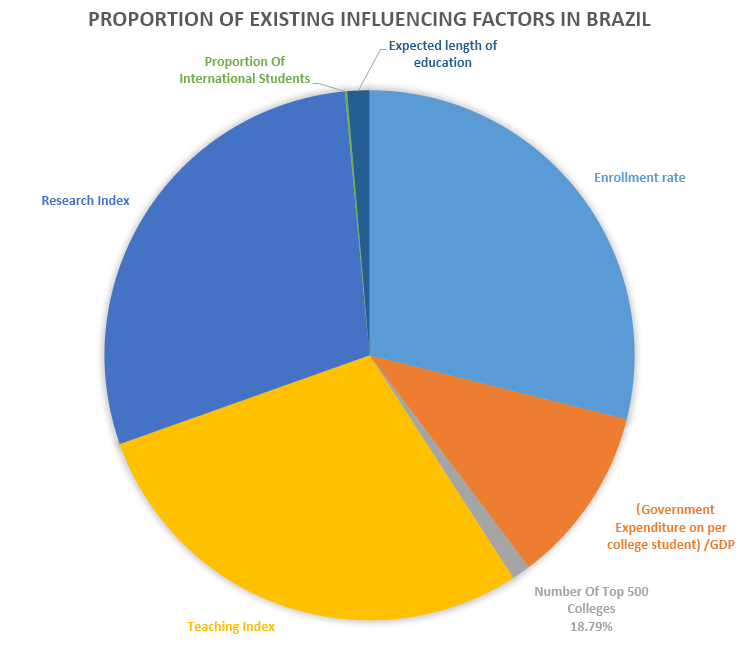
\includegraphics[width=\textwidth]{Proportion a.PNG}
		\caption{Now}
	\end{subfigure}
	\begin{subfigure}[b]{.4\textwidth}
		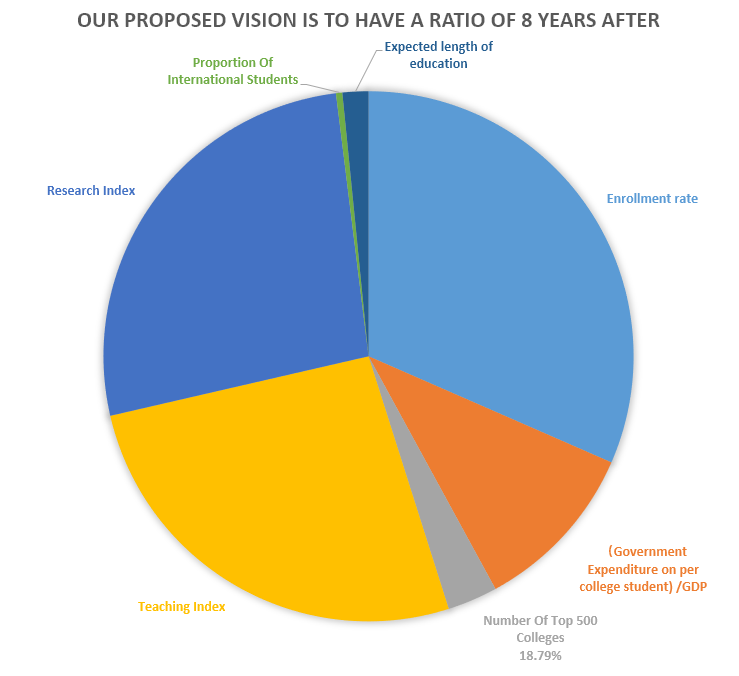
\includegraphics[width=\textwidth]{Proportion b.PNG}
		\caption{8 years later}
	\end{subfigure}
	\caption{Comparison}\label{fig:ccc}
\end{figure}

% 子图(多图并列)示例,更多用法请参考 subfigure 宏包文档
% 如果您只希望几张图并列,不需要额外的 caption,那么在 figure 环境中
% 连续插入总宽度不超过 \textwidth 的多个 \includegraphics 命令即可
\section {Proposed healthy sustainable system}
The changed data were brought into the model to produce the results and compared with the existing system as shown in Table \ref{tb:zzz}.
\begin{table}[htp]
	\begin{center}
		\caption{Comparison}
		\begin{tabular}{|c|c|c|}
			\hline
			& Proposed Sysytem & Current system \\ \hline
			Score            & 3.186            & 2.7872         \\ \hline
			Health Condition & Healthy          & normal         \\ \hline
		\end{tabular}\label{tb:zzz}
	\end{center}
	\end{table}
		
The proposed system is healthier and more sustainable than the existing system.
\section{Implementation Policy and Timetable}
According to the evaluation and assessment report, we find both the enrollment rate and years of education are on the low side, and the quality of colleges and universities is even lower with relatively high government spending on education. Thus, we mainly proposed the following policies(P) for these three areas:

$P_1$:Reduce the number of admissions reserved by the decree on the mandatory tilt of ENEM.

$P_2$:Encourage healthy competition among private universities and establish evaluation criteria for universities, with top universities receiving government financial incentives.

$P_3$:Strengthen the management of universities and introduce corresponding laws to prevent vicious competition arising from the allocation of educational resources.

$P_4$:Increase the number of universities by lowering the threshold for founding private universities and reorganization of existing public universities in Brazil to lower the entrance threshold.

$P_5$:Increase the ratio of enrolling graduate and doctoral students.
The policy implementation schedule is shown in the following Figure \ref{fig:ddd}

\begin{figure}[htp]
	\centering
	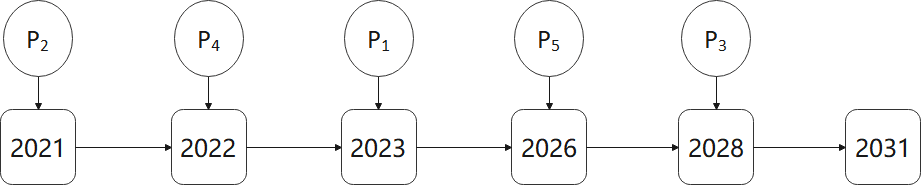
\includegraphics[width=.9\textwidth]{Policy.png}
	\caption{Implementation Timetable a}\label{fig:ddd}
\end{figure}

\section{Evaluate policy effectiveness}
\subsection{Establish a policy effectiveness evaluation model}
The relative implementation strength of policy$P_i(i=1,2,...5)$ is Equation \eqref{eq:kkk} 
\begin{equation}\label{eq:kkk}
W=(w_1,w_2,w_3,w_4,w_5)=(0.3,0.2,0.2,0.1,0.2)
\end{equation}

Construct the correlation matrix $N=(n_{ij})_{5\times7}$ between policy P and the influencing factor A: Matrix \eqref{eq:mmm}
\begin{equation}\label{eq:mmm}
N=\begin{pmatrix}
0.2&0&0.5&0.3&0&0&0\\
0&0.2&0.4&0.2&0.2&0&0\\
0.2&0&0.5&0.1&0.1&0&0\\
0.5&0.2&0&0.1&0&0.2&0\\
0&0&0.1&0.1&0.1&0.2&0.4\\
\end{pmatrix}
\end{equation}

The final Influence Matrix of $P$ on $A$is $D$\eqref{eq:nnn}
\begin{equation}\label{eq:nnn}
\begin{split}
D&=WN=(d_1,d_2,d_3,d_4,d_5,d_6,d_7)\\
D&=(0.1500,0.0600,0.3500,0.1800,0.0800,0.0600,0.0800)
\end{split}
\end{equation}

In 7, it is stated that $I_1,I_3,I_7$ need to be improved, especially for $I_3$. From the Influence Matrix of $P$ on $A$,$I_1$, $I_3$, and $I_7$ are affected by the implementation of new policies to the extent of 0.15, 0.35, and 0.08, respectively, with $I_3$ having the highest influence of all at 0.35. 

Thus, the implementation of the five new policies was very effective in improving the health of higher education in Brazil.
\subsection{Real-world impact of policy implementation}
1. The downward adjustment of the mandatory tilt decree policy will definitely harm the interests of low-income families, black and Indian students, and will also increase the polarization between rich and poor in Brazil.

2. The university merit system is not professional, comprehensive and careful assessment will be costly and laborious, and simple assessment will be easily exploited by some schools to obtain government incentive funds.

3. For developing countries where the gap between rich and poor is serious and the education level per capita is low, basic education should be developed vigorously to improve the quality of the general labor force. The expansion of graduate and doctoral students will make the problem more serious.

4. The liberalization of teaching qualifications in private universities will inevitably lead to the emergence of inferior universities and deepen citizens' perceptions of the polarization between public and private universities. The increase in profit-oriented private universities will also lead to a shift in national resources, and the education industry will hold more social resources.
\section{Strengths and Weaknesses}
\subsection{Strengths}
\begin{itemize}
    \item The data is rich in variety, and the grade boundaries are reasonably used to better reflect the essence.
    \item The use of models is reasonable and quantitative factors.
    \item Policies and schedules are formulated with real consideration of national conditions and are reasonable and effective.
\end{itemize}

\subsection{Weaknesses}
\begin{itemize}
    \item No classification of countries is discussed, and countries can be classified by GNI to build different models for evaluation.
    \item Few types of models, simple structure, can not make more accurate evaluation, can not make full use of data.
    \item The models are highly subjective, and many of them are for personal understanding, which affects the final evaluation results.
 \end{itemize}
 
% 参考文献,此处以 MLA 引用格式为例
\begin{thebibliography}{99}
	\bibitem{1} OECD (2021), "Education at a glance: Share of international students enrolled by field of education", OECD Education Statistics (database), \url{https://doi.org/10.1787/e86f4692-en (accessed on 06 February 2021)}.
	\bibitem{2}OECD (2019), "Education Database: Enrolment of international students by origin (Edition 2019/1)", OECD Education Statistics (database), \url{https://doi.org/10.1787/f5089015-en (accessed on 06 February 2021)}.
	\bibitem{3}\url{https://www.gov.br/inep/pt-br/areas-de-atuacao/avaliacao-e-exames-educacionais/enem}.
	\bibitem{4}World Education Database from the World UNESCO \url{https://zh.unesco.org/gem-report/node/13}.
	\bibitem{5}"Times Higher Education" from\url{https://www.timeshighereducation.com/}.
	\bibitem{6}Dong, Jun. "Analysis of hierarchical analysis method of weight calculation and its application research." Science and Technology Information v.13;No.422.29(2015):218-218.
	\bibitem{7}Kaiyou Yuan, Yuan Kaiyou, Li Heng, et al. Research on AHP-fuzzy comprehensive evaluation method and application. 2020, 1592(1):012045-.
	\bibitem{8}Y. C. Chou, H. Y. Yen, C. C. Sun and J. S. Hon, "Comparison of AHP and fuzzy AHP methods for human resources in science technology (HRST) performance index selection," 2013 IEEE International Conference on Industrial Engineering and Engineering Management, Bangkok, 2013, pp. 792-796, doi: 10.1109/IEEM.2013.6962520.
\end{thebibliography}

\end{document}  % 结束
